\tikzset{every picture/.style={line width=0.75pt}} %set default line width to 0.75pt

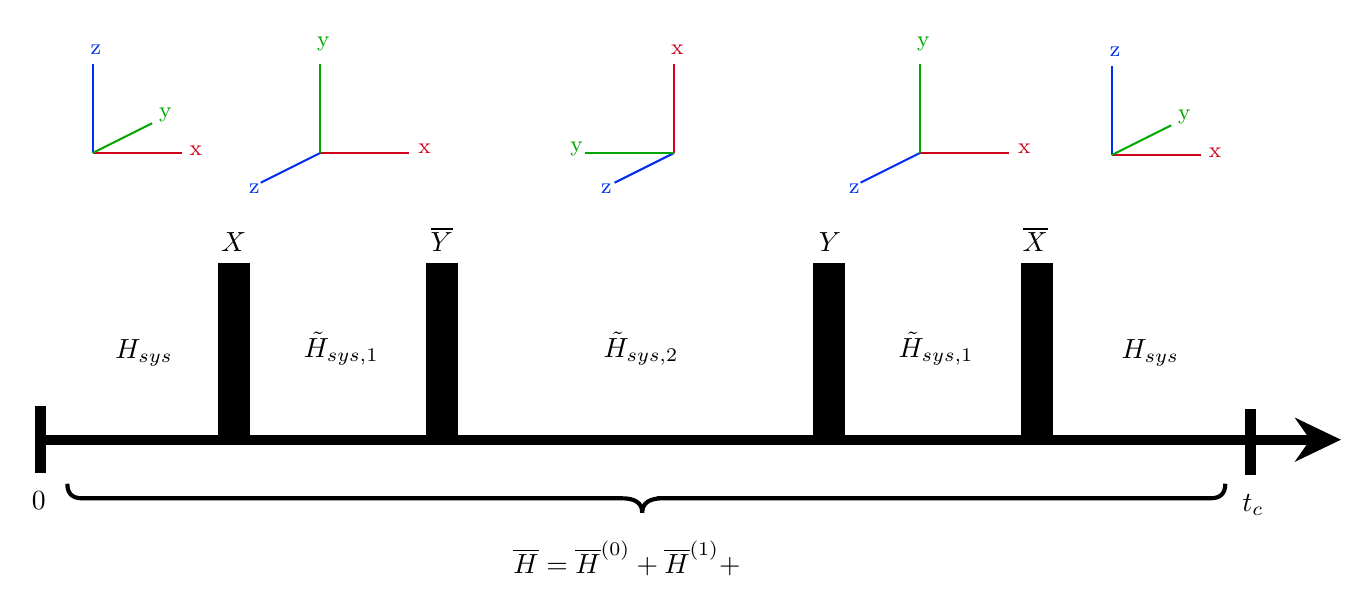
\begin{tikzpicture}[x=0.75pt,y=0.75pt,yscale=-1,xscale=1]
%uncomment if require: \path (0,327); %set diagram left start at 0, and has height of 327

%Shape: Rectangle [id:dp757529732417089]
\draw  [fill={rgb, 255:red, 0; green, 0; blue, 0 }  ,fill opacity=1 ] (101.1,123.91) -- (115.43,123.91) -- (115.43,209.89) -- (101.1,209.89) -- cycle ;
%Straight Lines [id:da8398663533091074]
\draw [line width=3.75]    (15.12,208.75) -- (634.62,208.75) ;
\draw [shift={(641.62,208.75)}, rotate = 180] [fill={rgb, 255:red, 0; green, 0; blue, 0 }  ][line width=0.08]  [draw opacity=0] (22.33,-10.72) -- (0,0) -- (22.33,10.73) -- (14.83,0) -- cycle    ;
%Shape: Rectangle [id:dp8989097393091372]
\draw  [fill={rgb, 255:red, 0; green, 0; blue, 0 }  ,fill opacity=1 ] (201.41,123.91) -- (215.74,123.91) -- (215.74,209.89) -- (201.41,209.89) -- cycle ;
%Shape: Rectangle [id:dp5203891268410358]
\draw  [fill={rgb, 255:red, 0; green, 0; blue, 0 }  ,fill opacity=1 ] (387.69,123.91) -- (402.02,123.91) -- (402.02,209.89) -- (387.69,209.89) -- cycle ;
%Shape: Rectangle [id:dp5922766644502158]
\draw  [fill={rgb, 255:red, 0; green, 0; blue, 0 }  ,fill opacity=1 ] (488,123.91) -- (502.33,123.91) -- (502.33,209.89) -- (488,209.89) -- cycle ;
%Shape: Brace [id:dp004729490444473794]
\draw  [line width=1.5]  (28.02,229.96) .. controls (28.02,234.63) and (30.35,236.96) .. (35.02,236.96) -- (295,236.96) .. controls (301.67,236.96) and (305,239.29) .. (305,243.96) .. controls (305,239.29) and (308.33,236.96) .. (315,236.96)(312,236.96) -- (578.92,236.96) .. controls (583.59,236.96) and (585.92,234.63) .. (585.92,229.96) ;
%Straight Lines [id:da5692356671850871]
\draw [color={rgb, 255:red, 208; green, 2; blue, 27 }  ,draw opacity=1 ]   (40.21,70.6) -- (83.2,70.6) ;
%Straight Lines [id:da6810769300954256]
\draw [color={rgb, 255:red, 0; green, 47; blue, 241 }  ,draw opacity=1 ]   (40.21,70.6) -- (40.21,27.61) ;
%Straight Lines [id:da050165915493954216]
\draw [color={rgb, 255:red, 0; green, 167; blue, 0 }  ,draw opacity=1 ]   (40.21,70.6) -- (68.87,56.27) ;

%Straight Lines [id:da5081204556289702]
\draw [color={rgb, 255:red, 208; green, 2; blue, 27 }  ,draw opacity=1 ]   (149.82,70.6) -- (192.81,70.6) ;
%Straight Lines [id:da6854547629628449]
\draw [color={rgb, 255:red, 0; green, 47; blue, 241 }  ,draw opacity=1 ]   (149.82,70.6) -- (121.16,84.93) ;
%Straight Lines [id:da7186146502407351]
\draw [color={rgb, 255:red, 0; green, 167; blue, 0 }  ,draw opacity=1 ]   (149.82,70.6) -- (149.82,27.61) ;

%Straight Lines [id:da24563094299910881]
\draw [color={rgb, 255:red, 208; green, 2; blue, 27 }  ,draw opacity=1 ]   (320.34,70.6) -- (320.34,27.61) ;
%Straight Lines [id:da179977702531384]
\draw [color={rgb, 255:red, 0; green, 47; blue, 241 }  ,draw opacity=1 ]   (320.34,70.6) -- (291.68,84.93) ;
%Straight Lines [id:da7516580599441232]
\draw [color={rgb, 255:red, 0; green, 167; blue, 0 }  ,draw opacity=1 ]   (320.34,70.6) -- (277.35,70.6) ;

%Straight Lines [id:da5137007458732086]
\draw [line width=3.75]    (598.05,193.84) -- (598.05,225.94) ;
%Straight Lines [id:da9300296101367684]
\draw [line width=3.75]    (15.12,192.7) -- (15.12,224.8) ;
%Straight Lines [id:da0881233734207878]
\draw [color={rgb, 255:red, 208; green, 2; blue, 27 }  ,draw opacity=1 ]   (531.21,71.6) -- (574.2,71.6) ;
%Straight Lines [id:da9374652913281989]
\draw [color={rgb, 255:red, 0; green, 47; blue, 241 }  ,draw opacity=1 ]   (531.21,71.6) -- (531.21,28.61) ;
%Straight Lines [id:da610003280154453]
\draw [color={rgb, 255:red, 0; green, 167; blue, 0 }  ,draw opacity=1 ]   (531.21,71.6) -- (559.87,57.27) ;

%Straight Lines [id:da5081271261395761]
\draw [color={rgb, 255:red, 208; green, 2; blue, 27 }  ,draw opacity=1 ]   (438.82,70.6) -- (481.81,70.6) ;
%Straight Lines [id:da9429921450367487]
\draw [color={rgb, 255:red, 0; green, 47; blue, 241 }  ,draw opacity=1 ]   (438.82,70.6) -- (410.16,84.93) ;
%Straight Lines [id:da28825440756966425]
\draw [color={rgb, 255:red, 0; green, 167; blue, 0 }  ,draw opacity=1 ]   (438.82,70.6) -- (438.82,27.61) ;


% Text Node
\draw (108.11,113.73) node  [font=\normalsize] [align=left] {$\displaystyle X$};
% Text Node
\draw (208.42,112.3) node  [font=\normalsize] [align=left] {$\displaystyle \overline{Y}$};
% Text Node
\draw (494.3,112.3) node  [font=\normalsize] [align=left] {$\displaystyle \overline{X}$};
% Text Node
\draw (395.43,113.73) node  [font=\normalsize] [align=left] {$\displaystyle Y$};
% Text Node
\draw (592.63,233.46) node [anchor=north west][inner sep=0.75pt]  [font=\normalsize]  {$t_{c}$};
% Text Node
\draw (9.41,232.39) node [anchor=north west][inner sep=0.75pt]  [font=\normalsize]  {$0$};
% Text Node
\draw (64.99,166.9) node  [font=\normalsize]  {$H_{\text{sys}}$};
% Text Node
\draw (160,164.75) node  [font=\normalsize]  {$\tilde{H}_{\text{sys, 1}}$};
% Text Node
\draw (304.44,164.75) node  [font=\normalsize]  {$\tilde{H}_{\text{sys, 2}}$};
% Text Node
\draw (446.59,164.75) node  [font=\normalsize]  {$\tilde{H}_{\text{sys, 1}}$};
% Text Node
\draw (549.77,166.9) node  [font=\normalsize]  {$H_{\text{sys}}$};
% Text Node
\draw (241.4,256.21) node [anchor=north west][inner sep=0.75pt]  [font=\normalsize]  {$\overline{H} =\overline{H}^{( 0)} +\overline{H}^{( 1)} +\dotsc $};
% Text Node
\draw (89.95,69.6) node  [font=\footnotesize,color={rgb, 255:red, 208; green, 2; blue, 27 }  ,opacity=1 ] [align=left] {x};
% Text Node
\draw (75.19,52.4) node  [font=\footnotesize,color={rgb, 255:red, 0; green, 167; blue, 0 }  ,opacity=1 ] [align=left] {y};
% Text Node
\draw (41.79,20.87) node  [font=\footnotesize,color={rgb, 255:red, 0; green, 47; blue, 241 }  ,opacity=1 ] [align=left] {z};
% Text Node
\draw (200.12,68.6) node  [font=\footnotesize,color={rgb, 255:red, 208; green, 2; blue, 27 }  ,opacity=1 ] [align=left] {x};
% Text Node
\draw (151.4,18.01) node  [font=\footnotesize,color={rgb, 255:red, 0; green, 167; blue, 0 }  ,opacity=1 ] [align=left] {y};
% Text Node
\draw (118.16,87.93) node  [font=\footnotesize,color={rgb, 255:red, 0; green, 47; blue, 241 }  ,opacity=1 ] [align=left] {z};
% Text Node
\draw (321.93,20.87) node  [font=\footnotesize,color={rgb, 255:red, 208; green, 2; blue, 27 }  ,opacity=1 ] [align=left] {x};
% Text Node
\draw (273.35,68.6) node  [font=\footnotesize,color={rgb, 255:red, 0; green, 167; blue, 0 }  ,opacity=1 ] [align=left] {y};
% Text Node
\draw (287.68,87.93) node  [font=\footnotesize,color={rgb, 255:red, 0; green, 47; blue, 241 }  ,opacity=1 ] [align=left] {z};
% Text Node
\draw (407.16,87.93) node  [font=\footnotesize,color={rgb, 255:red, 0; green, 47; blue, 241 }  ,opacity=1 ] [align=left] {z};
% Text Node
\draw (440.4,18.01) node  [font=\footnotesize,color={rgb, 255:red, 0; green, 167; blue, 0 }  ,opacity=1 ] [align=left] {y};
% Text Node
\draw (489.12,68.6) node  [font=\footnotesize,color={rgb, 255:red, 208; green, 2; blue, 27 }  ,opacity=1 ] [align=left] {x};
% Text Node
\draw (532.79,21.87) node  [font=\footnotesize,color={rgb, 255:red, 0; green, 47; blue, 241 }  ,opacity=1 ] [align=left] {z};
% Text Node
\draw (566.19,53.4) node  [font=\footnotesize,color={rgb, 255:red, 0; green, 167; blue, 0 }  ,opacity=1 ] [align=left] {y};
% Text Node
\draw (580.95,70.6) node  [font=\footnotesize,color={rgb, 255:red, 208; green, 2; blue, 27 }  ,opacity=1 ] [align=left] {x};


\end{tikzpicture}
